\documentclass{article}
\usepackage[pdfcreator={LaTeX}]{hyperref}
\usepackage{graphicx}
\usepackage[utf8]{inputenc} 
\usepackage[ngerman]{babel}


\usepackage{tikz}
\usetikzlibrary{arrows,shadows}
\usepackage{pgf-umlsd}


\begin{document}
\begin{titlepage}

\begin{center}
\textbf{\textsc{\LARGE Spezifikation}}

{\large \today}

\vspace{2cm}
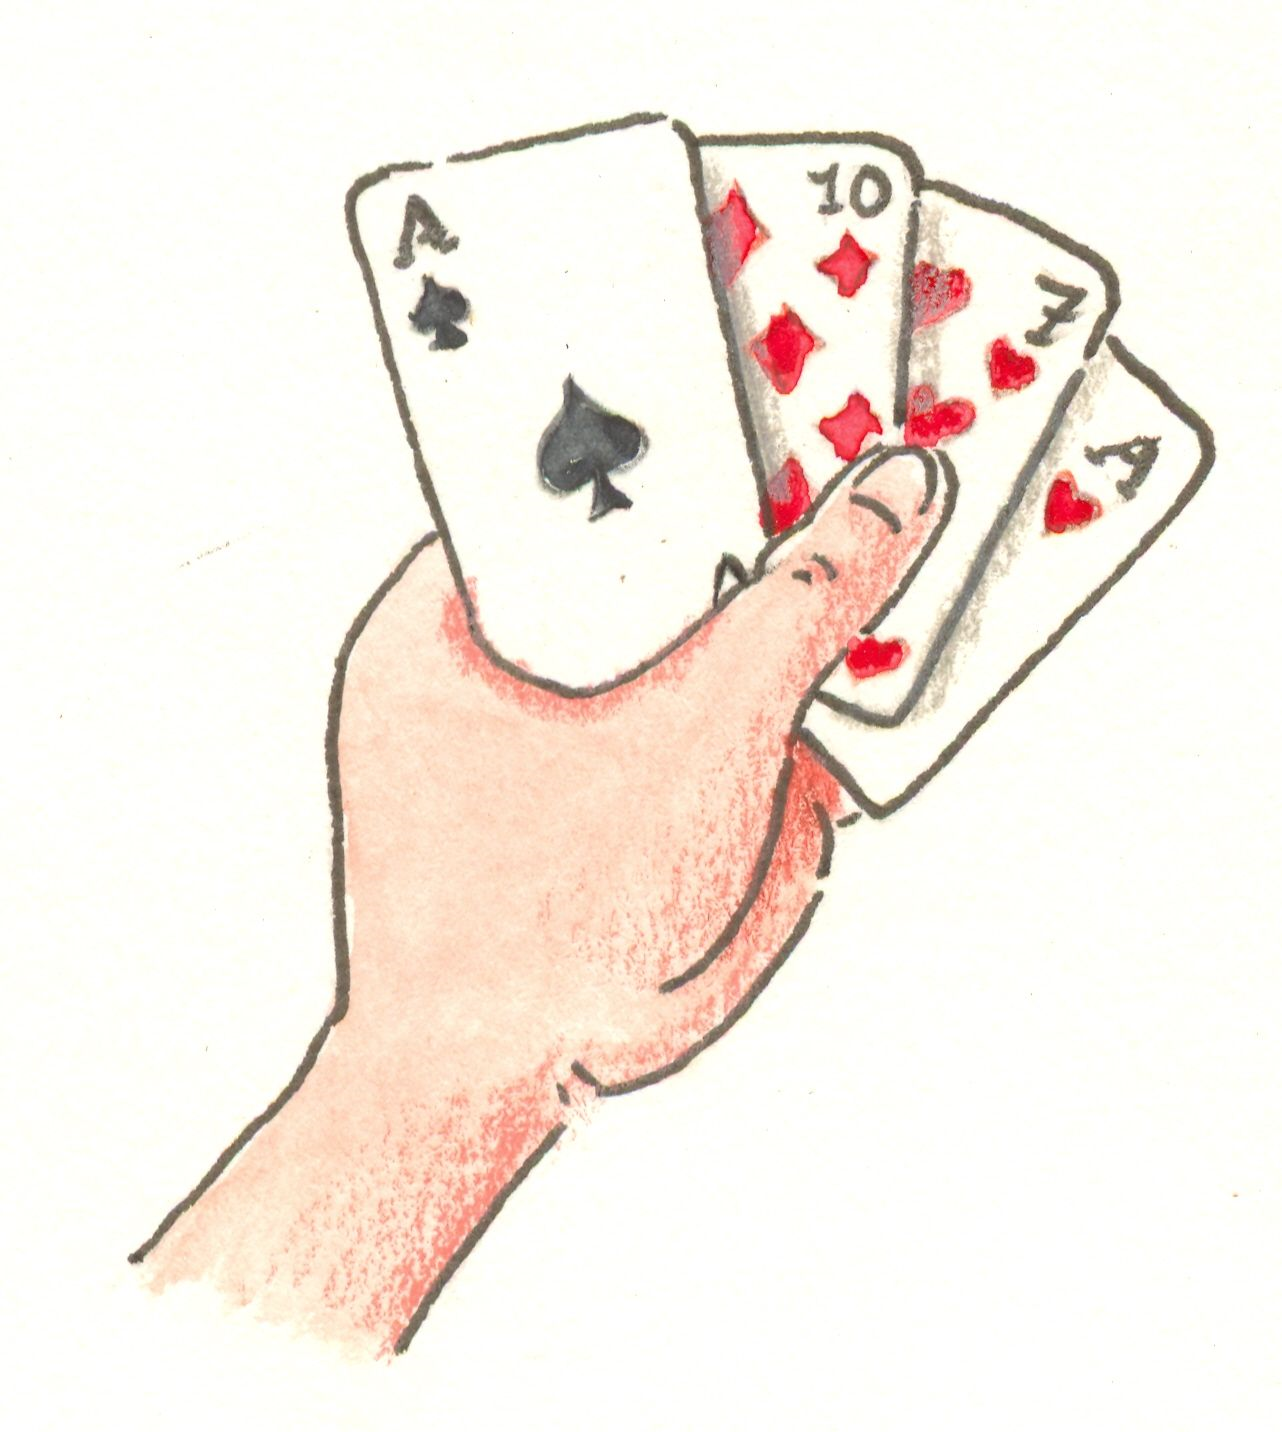
\includegraphics{kartenspiel}
\ \\
\ \\

\textbf{\textsc{\LARGE NET-WizHearts}}
\vspace{2cm}

\begin{tabular}{|c|c|c|}\hline
   Phase & Verantwortlicher & E-Mail \\ \hline\hline
   Pflichtenheft & Alina Meixl &  alina@meixl.de \\ \hline
   Entwurf & Viktoria Witka & witkaviktoria@freenet.de \\ \hline
   Spezifikation & Daniel Riedl & dariedl14@yahoo.de \\ \hline
   Implementation & Andreas Altenbuchner& a.andi007@gmail.com\\ \hline
   Verifikation & Patrick Kubin & kubin@fim.uni-passau.de\\ \hline
   Präsentation & w& w\\ \hline
 \end{tabular}

\end{center}

\end{titlepage}

\tableofcontents
\newpage

\section{Einleitung}
Hier kommt die Spezifikation.
\  \\


\section{Systemarchitektur}
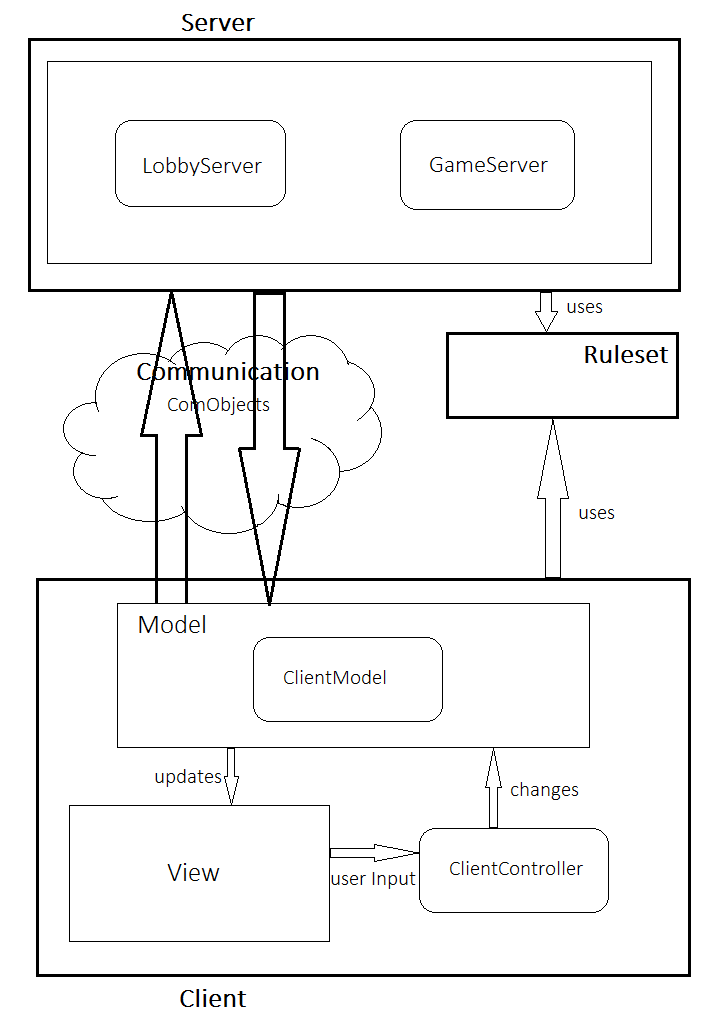
\includegraphics[width=\textwidth]{ArchitekturDiagramm}
\newpage

\section{Klassendiagramm}

\subsection{Packages}
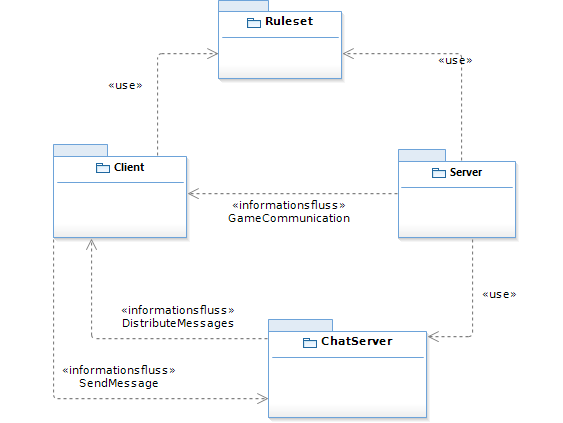
\includegraphics[width=\textwidth]{Packages}
\newpage

\section{Änderungen am Entwurf}
\subsection{Zusätzliche Pattern}
\subsubsection{Factory Pattern}
Objekte erstellen, Messages
\subsubsection{Builder Pattern}
Zum zeichnen der Karten
\subsubsection{Visitor Pattern}
...

\subsection{Server}
Der Server war zuletzt ein Interface. Wir haben uns dennoch entschieden die Serverklasse als abstrakte Klasse zu schreiben. So können die Methoden an die 'unteren' Server vererbt werden und wenn nötig überschrieben. Auch die Aggregagtion stimmt somit wieder.
\subsection{}
\subsection{}
\subsection{}
\subsection{}
\newpage

\section{Spezifizierung der Klassen}
\subsection{Client}
Methoden
Attribute
Beschreibung

Gespeichterte Daten?? für Karten
\subsubsection{ClientMain}
\subsubsection{ClientController}
\subsubsection{ClientModel}
\subsubsection{MessageListenerThread}
\subsubsection{MVMessage}
\subsubsection{MVLobby}
\subsubsection{MVGameLobby}
\subsubsection{MVGame}
\subsubsection{Window}
\subsubsection{WizID}
\subsubsection{HeartsID}
\newpage

\subsection{View}
\subsubsection{Lobby}
\subsubsection{GameLobby}
\subsubsection{Game}
\subsubsection{Password}
\subsubsection{CreateGame}
\subsubsection{Login}
\subsubsection{ChooseItem}
\subsubsection{Warning}
\subsubsection{InputNumber}
\subsubsection{MVMessages}
\subsubsection{ScoreWindow}
\subsubsection{ChooseCards}
\subsubsection{GamePanel}
\subsubsection{DiscardPile}
\subsubsection{DrawDesk}
\subsubsection{OtherPlayer}
\subsubsection{OwnHand}
\subsubsection{Language}
\newpage

\subsection{Ruleset}
\subsubsection{ServerRuleset}
\subsubsection{Wizard}
\subsubsection{Hearts}
\subsubsection{GameState}
\subsubsection{GameClientUpdate}
\subsubsection{HeartsData}
\subsubsection{WizData}
\subsubsection{PlayerState}
\subsubsection{Card}
\subsubsection{OtherData}
\subsubsection{GamePhase}
\subsubsection{WizardCard}
\subsubsection{HeartsCard}
\newpage

\subsection{Server}
\subsubsection{ServerMain}
\subsubsection{LobbyServer}
\subsubsection{GameServer}
\subsubsection{ClientListenerThread}
\subsubsection{GameServer}
\subsubsection{Server}
\subsubsection{Player}
\subsubsection{GameServerRepräsentation}
\newpage

\subsection{ComObjects}
\subsubsection{Ruleset}
\subsubsection{ComObject}
\subsubsection{Commands}
\subsubsection{ComLogin}
\subsubsection{ComUpdatePlayerlist}
\subsubsection{ComInitGameLobby}
\subsubsection{ComChatMessage}
\subsubsection{ComPassword}
\subsubsection{ComJoinRequest}
\subsubsection{ComKicklayer}
\subsubsection{ComInitGameLobby}
\subsubsection{ComLobbyUpdateGamelist}
\newpage

\section{JUnit-Tests}
\newpage

\section{Implementierungsplan}
Es werden für jeden Milestone die einzelnen Arbeitspakete angegeben. Die angegebenen Klassen werden nicht sofort vollständig implmentiert, sondern mit den vom Arbeitspaket und Milestone verlangten Funktionen ausgestattet.\\

\subsection{Milestone 1}
Für den ersten Milestone werden folgende Funktionen angestrebt:\\
Der Nutzer kann sich im Login-Fenster anmelden und die Lobby betreten. Er kann ein Spiel erstellen und offenen Spielen beitreten. Das wird in der Lobby angezeigt, man gelangt jedoch noch nicht ins Wartefenster. Nebenläufig dazu wird die Datenschicht der Regelwerke implementiert.\\ 
\begin{itemize}
\item View(Login+Lobby) Dauer: 8 Std. \\
Klassen: Login, Lobby, Warning, ClientController
\item Client(Login) Dauer 8 Std. \\
Klassen: ClientMain, ClientModel, MessageListener Thread, ClientState, ViewNotification
\item Server(Login) Dauer 16 Std. \\
Klassen: Server, ServerMain, LobbyServer, Player, ClientListenerThread, ComObject, ComLoginRequest, ComClientQuit, ComServerAcknowledgement, ComWarning
\item Ruleset(Daten) Dauer 20 Std. \\
Klassen:  Card, Colour, HeartsCard, WizCard, OtherData, WizData, HeartsData, GameClientUpdate, GameState, PlayerState, RulesetType
\item Client(Lobby) Dauer 8 Std. \\
Klassen: ClientModel
\item Server(Lobby) Dauer 8 Std. \\
Klassen: LobbyServer, ComChatMessage, ComLobbyUpdateGamelist, ComJoinRequest, ComInitLobby, ComUpdatePlayerlist
\item View(Create+Join) Dauer 8 Std. \\
Klassen: Password, CreateGame, ClientController
\item Client(Create+Join) Dauer 8 Std. \\
Klassen: ClientModel
\item Server(Create+Join) Dauer 12 Std. \\
Klassen: LobbyServer, ComJoinRequest, ComCreateGameRequest
\end{itemize}

\subsection{Milestone 2}
Für den zweiten Milestone werden folgende Funktionen angestrebt:\\
Beim Beitreten oder Erstellen eines Spiels gelangt man ins Wartefenster. Der Spielleiter kannn hier Spieler entfernen. Diese gelangen zurück in die Lobby. Das Spiel kann noch nicht gestartet werden, aber das Regelwerk wird bereits serverseitig implementiert.\\
\begin{itemize}
\item Ruleset(Wizard-Server) Dauer 30 Std. \\
Klassen: ServerRuleset, ServerWizard, RulesetMessage, MsgCard, MsgCardRequest, MsgGameEnd, MsgNumber, Msg NumberRequest, MsgSelection, MsgSelectionRequest, MsgUser
\item View(GameLobby) Dauer 8 Std. \\
Klassen: GameLobby, ClientController
\item Client(GameLobby) Dauer 8 Std. \\
Klassen: ClientModel
\item Server(GameLobby) Dauer 10 Std. \\
KLassen: LobbyServer, GameServer, ComBeenKicked, ComClientLeave, ComInitGameLobby, ComKickPlayerRequest, ComStartGame
\item View(Game) Dauer 20 Std. \\
Klassen: Game, GamePanel, OtherPlayer, OwnHand, ViewCard, DrawDeck, DiscardPile, ScoreWindow, ClientController
\item Client(Game) Dauer 14 Std. \\
Klassen: ClientModel
\end{itemize}

\subsection{Milestone 3}
Für den dritten Milestone werden folgende Funktionen angestrebt:\\
Es kann schon eine vollständige Partie Wizard gespielt werden.\\
\begin{itemize}
\item Server(Game) Dauer 4 Std. \\
Klassen: GameServer, ComStartGame, ComRuleset, ComGameEnd
\item Ruleset(Wizard-Client) Dauer 12 Std. \\
Klassen: ClientWizard
\item View(WizardWindows) Dauer 4 Std. \\
Klassen: ChooseItem, InputNumber, ClientController
\item Client(Wizard) Dauer 6 Std. \\
Klassen: ClientModel
\item View(HeartsWindows) Dauer 2 Std. \\
Klassen: ChooseCards, ClientController
\item Client(Hearts) Dauer 4 Std. \\
Klassen: ClientModel
\item Ruleset(Hearts-Server) Dauer 16 Std. \\
Klassen: ServerHearts
\end{itemize}

\subsection{Finale Version}
Die finale Version enthält die volle Funktionalität des Programs.
Es können also sowohl Wizard als auch Hearts gespielt werden.\\
\begin{itemize}
\item Ruleset(Hearts-Client) Dauer 10Std. \\
Klassen: ClientHearts
\item ViewPolishing(evtl Tests) Dauer 10Std \\
Verbesserungen an der bisherigen Implementierung. Gegebenfalls Schreiben von zusätzlichen Tests
\item ClientPolishing(evtl Tests) Dauer 10Std \\
Verbesserungen an der bisherigen Implementierung. Gegebenfalls Schreiben von zusätzlichen Tests
\item ServerPolishing(evtl Tests) Dauer 10Std \\
Verbesserungen an der bisherigen Implementierung. Gegebenfalls Schreiben von zusätzlichen Tests
\item RulesetPolishing(evtl Tests) Dauer 10Std \\
Verbesserungen an der bisherigen Implementierung. Gegebenfalls Schreiben von zusätzlichen Tests
\end{itemize}
\newpage

\subsection{Gantt-Diagramme}
\hspace*{-0.2\textwidth}Milestone 1: \\ \\
\hspace*{-0.2\textwidth}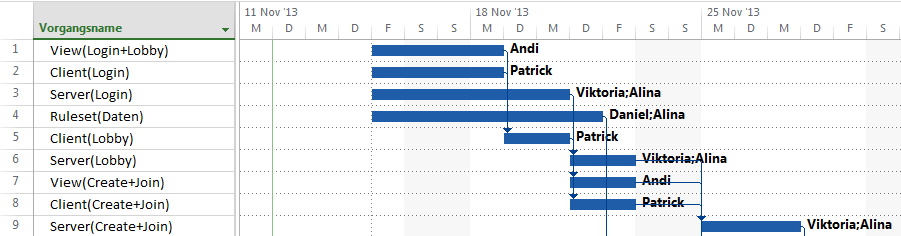
\includegraphics[width=1.4\textwidth]{Milestone1} \\ \\

\hspace*{-0.2\textwidth}Milestone 2: \\ \\
\hspace*{-0.2\textwidth}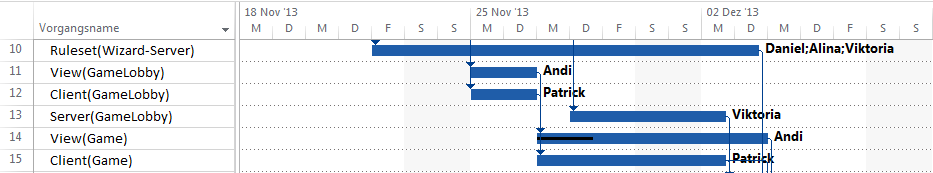
\includegraphics[width=1.4\textwidth]{Milestone2} \\ \\

\hspace*{-0.2\textwidth}Milestone 3: \\ \\
\hspace*{-0.2\textwidth}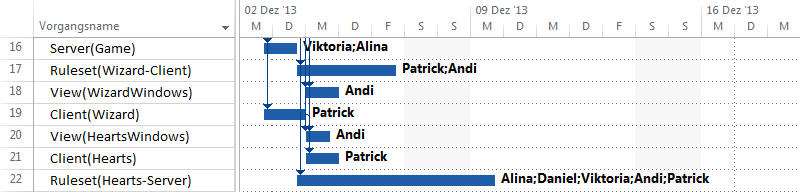
\includegraphics[width=1.4\textwidth]{Milestone3} \\ \\

\hspace*{-0.2\textwidth}Finale Version: \\ \\
\hspace*{-0.2\textwidth}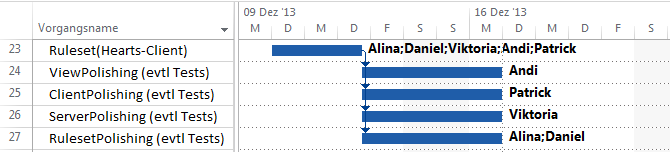
\includegraphics[width=1.4\textwidth]{Milestone4} \\ \\

\end{document}
